\documentclass[12pt, twoside]{article}
\usepackage[letterpaper, margin=1in, headsep=0.5in]{geometry}
\usepackage[english]{babel}
\usepackage[utf8]{inputenc}
\usepackage{amsmath}
\usepackage{amsfonts}
\usepackage{amssymb}
\usepackage{tikz}
\usetikzlibrary{quotes, angles}
\usepackage{graphicx}
%\usepackage{pgfplots}
%\pgfplotsset{width=10cm,compat=1.9}
%\usepgfplotslibrary{statistics}
%\usepackage{pgfplotstable}
%\usepackage{tkz-fct}
%\usepackage{venndiagram}

\usepackage{fancyhdr}
\pagestyle{fancy}
\fancyhf{}

\fancyhead[LE]{\thepage}
\fancyhead[RO]{\thepage \\ Name: \hspace{4cm} \, \\}
\fancyhead[LO]{BECA / Dr. Huson / Geometry 10th Grade\\* Unit 5: Transformation, dilation, \& scale \\ 4 November 2019}

\renewcommand{\headrulewidth}{0pt}

\begin{document}
\subsubsection*{5.1 Classwork: Construction of a dilation}
Use only a compass and straightedge for these classical constructions.
  \begin{enumerate}

  \item Construct a line segment $\overline{AB'}$ that is twice the length of $\overline{AB}$, $AB' = 2 \times AB$. \\ (Do not measure with a ruler. Leave all construction marks.)
    \vspace{1cm}
    \begin{center}
    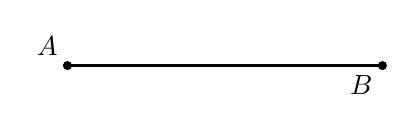
\begin{tikzpicture}
      \draw [-, thick] (0,0)--(4,0);
      \draw [fill] (0,0) circle [radius=0.05] node[above left]{$A$};
      \draw [fill] (4,0) circle [radius=0.05] node[below left]{$B$};
    \end{tikzpicture}
    \end{center}
    \vspace{3cm}

  \item Construct a triangle $\triangle AB'C'$ with sides twice the length of $\triangle ABC$, that is $AB' = 2 \times AB$, $AC' = 2 \times AC$, and $B'C' = 2 \times BC$.
    \vspace{5cm}
    \begin{flushleft}
    \begin{tikzpicture}
      \draw [-, thick] (0,0)--(6,0)--(6,4)--cycle;
      \draw [fill] (0,0) circle [radius=0.05] node[left]{$A$};
      \draw [fill] (6,0) circle [radius=0.05] node[below]{$B$};
      \draw [fill] (6,4) circle [radius=0.05] node[above left]{$C$};
    \end{tikzpicture}
  \end{flushleft} 

\newpage
\subsubsection*{Dilate a triangle with a center of dilation}
  \item Perform a dilation centered at $P$ with a scale factor $k=2$. \\
  Make a table of the two triangles' side lengths, showing their ratios.
      \vspace{5cm}
      \begin{center}
      \begin{tikzpicture}[scale=0.7]
        \draw [<->, thick] (0,0) node[below right]{$A$}--
        (9,0) node[below left]{$C$}--
        (7,11) node[right]{$B$}--cycle;
        \draw [fill] (6, 6) circle [radius=0.05] node[right]{$P$};
      \end{tikzpicture}
      \end{center}


\end{enumerate}
\end{document}
